\chapter{Implementation}
\label{details}
The required constants, generics and types for this project are contained in one main package called \texttt{dlx\_utils}, which must always be compiled as the first entry. All the entities described below inherently depend on it, while also making use of the standard \texttt{IEEE} library (with the exception of Memories, which include \texttt{STD} as well).

\section{Fundamental blocks}
The implementation of the DLX followed a bottom-up approach in which the lowest level building blocks were to be instantiated first. In the following, they are listed in alphabetical order.

\subsection{\texttt{alu}}
This behavioral unit mainly consists in one prominent \texttt{CASE} statement, whose branches are managed by an \texttt{ALU\_MSG} special signal. The latter is an enumerated type representing all the possible operations linked to the Instruction Set. An internal variable with a 33rd additional bit is used to compute and handle both the result and some condition code flags. Of course, the block in question is wholly fault-tolerant.

It's important to notice that two operations were added (\texttt{R\_mult} and \texttt{R\_multu}) in order for them to work with an integer register file: their OPCODE was switched from \texttt{0x01} to \texttt{0x00} while the corresponding FUNC remained tha same, as to effectively convert them from FP to R-Type. In this context, both input operands had to be (equally) truncated to Half Word length in order to generate a result on 32-bits only.

\begin{figure}[!ht]
\centering
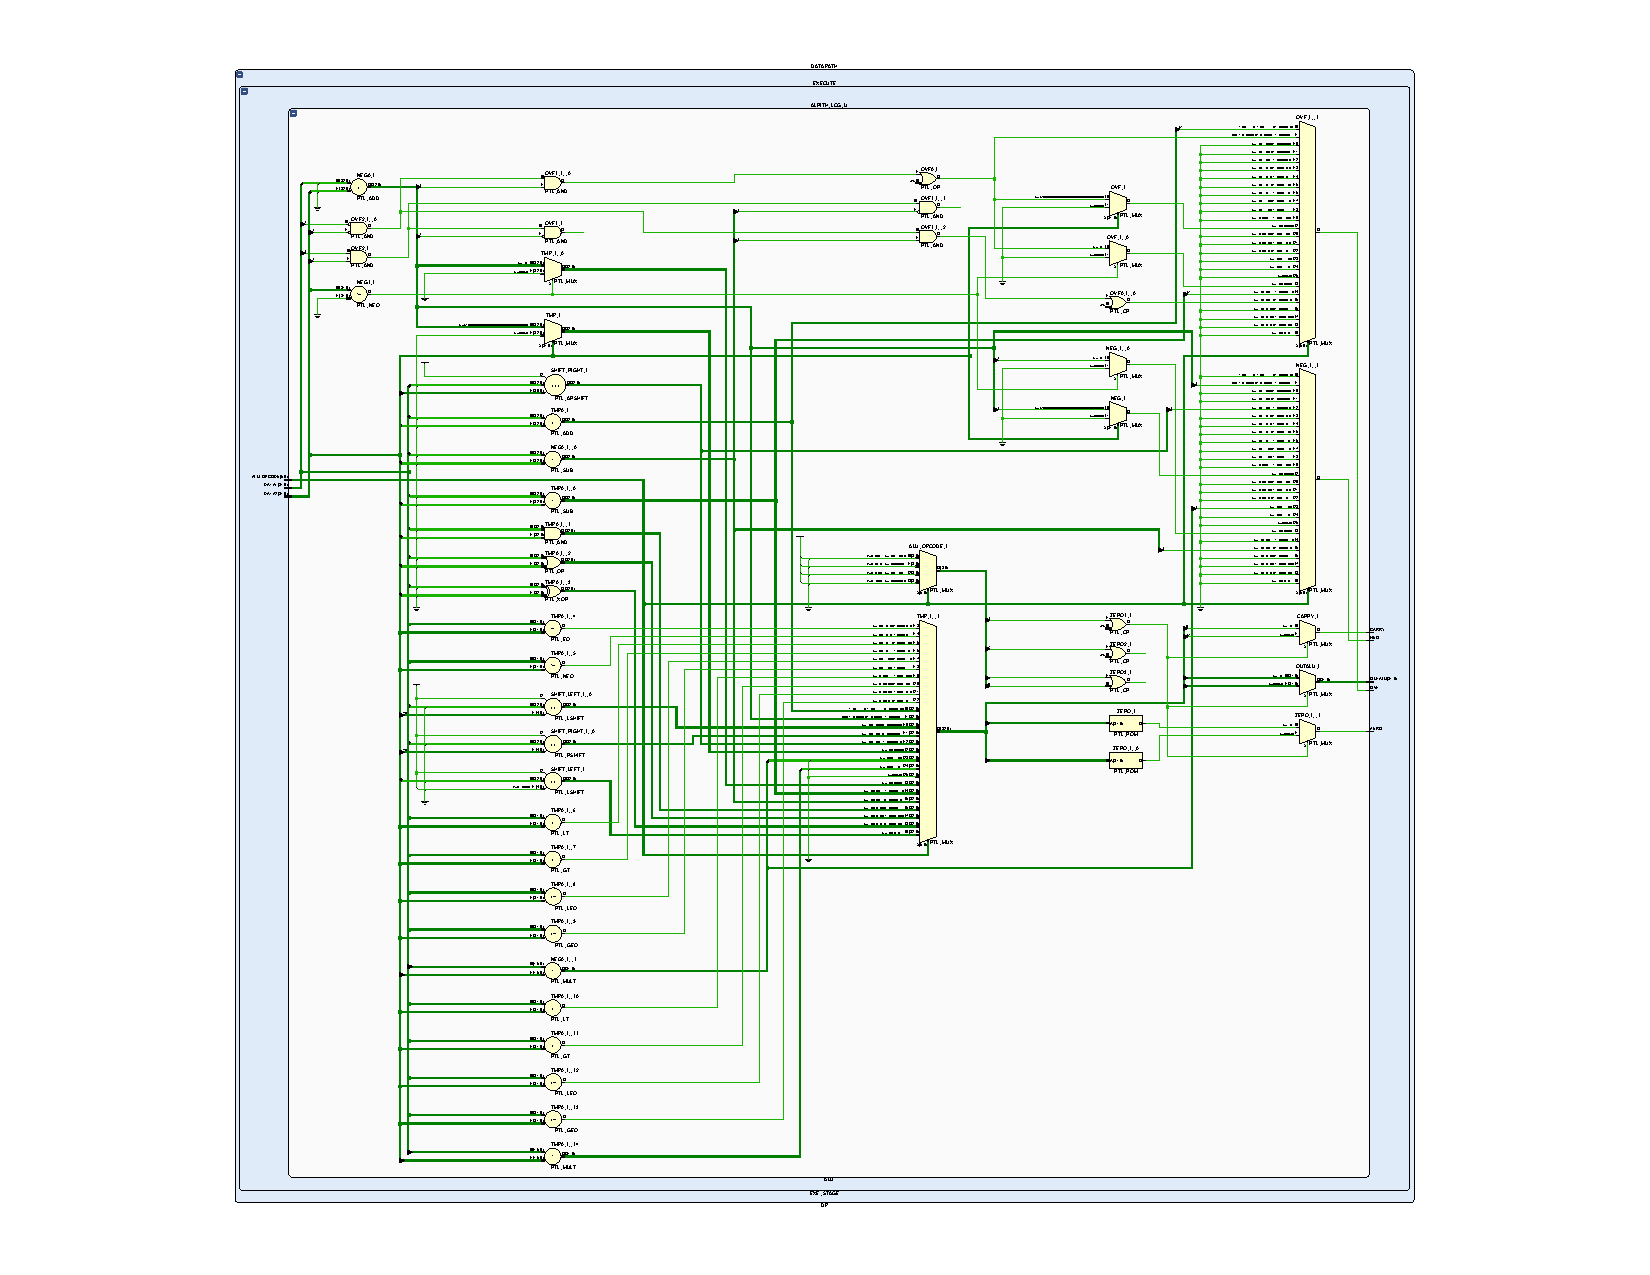
\includegraphics[width=\textwidth]{./chapters/figures/alu.pdf} 
\caption{Schematic of the behavioral \texttt{alu}.}
\end{figure}

\subsection{\texttt{cond\_branch}}
\label{cond-branch}
A combinational set of two logic gates used to determine whether to perform a branch or not, with a dataflow description that directly optimizes the intended behavior.

\begin{figure}[!ht]
\centering
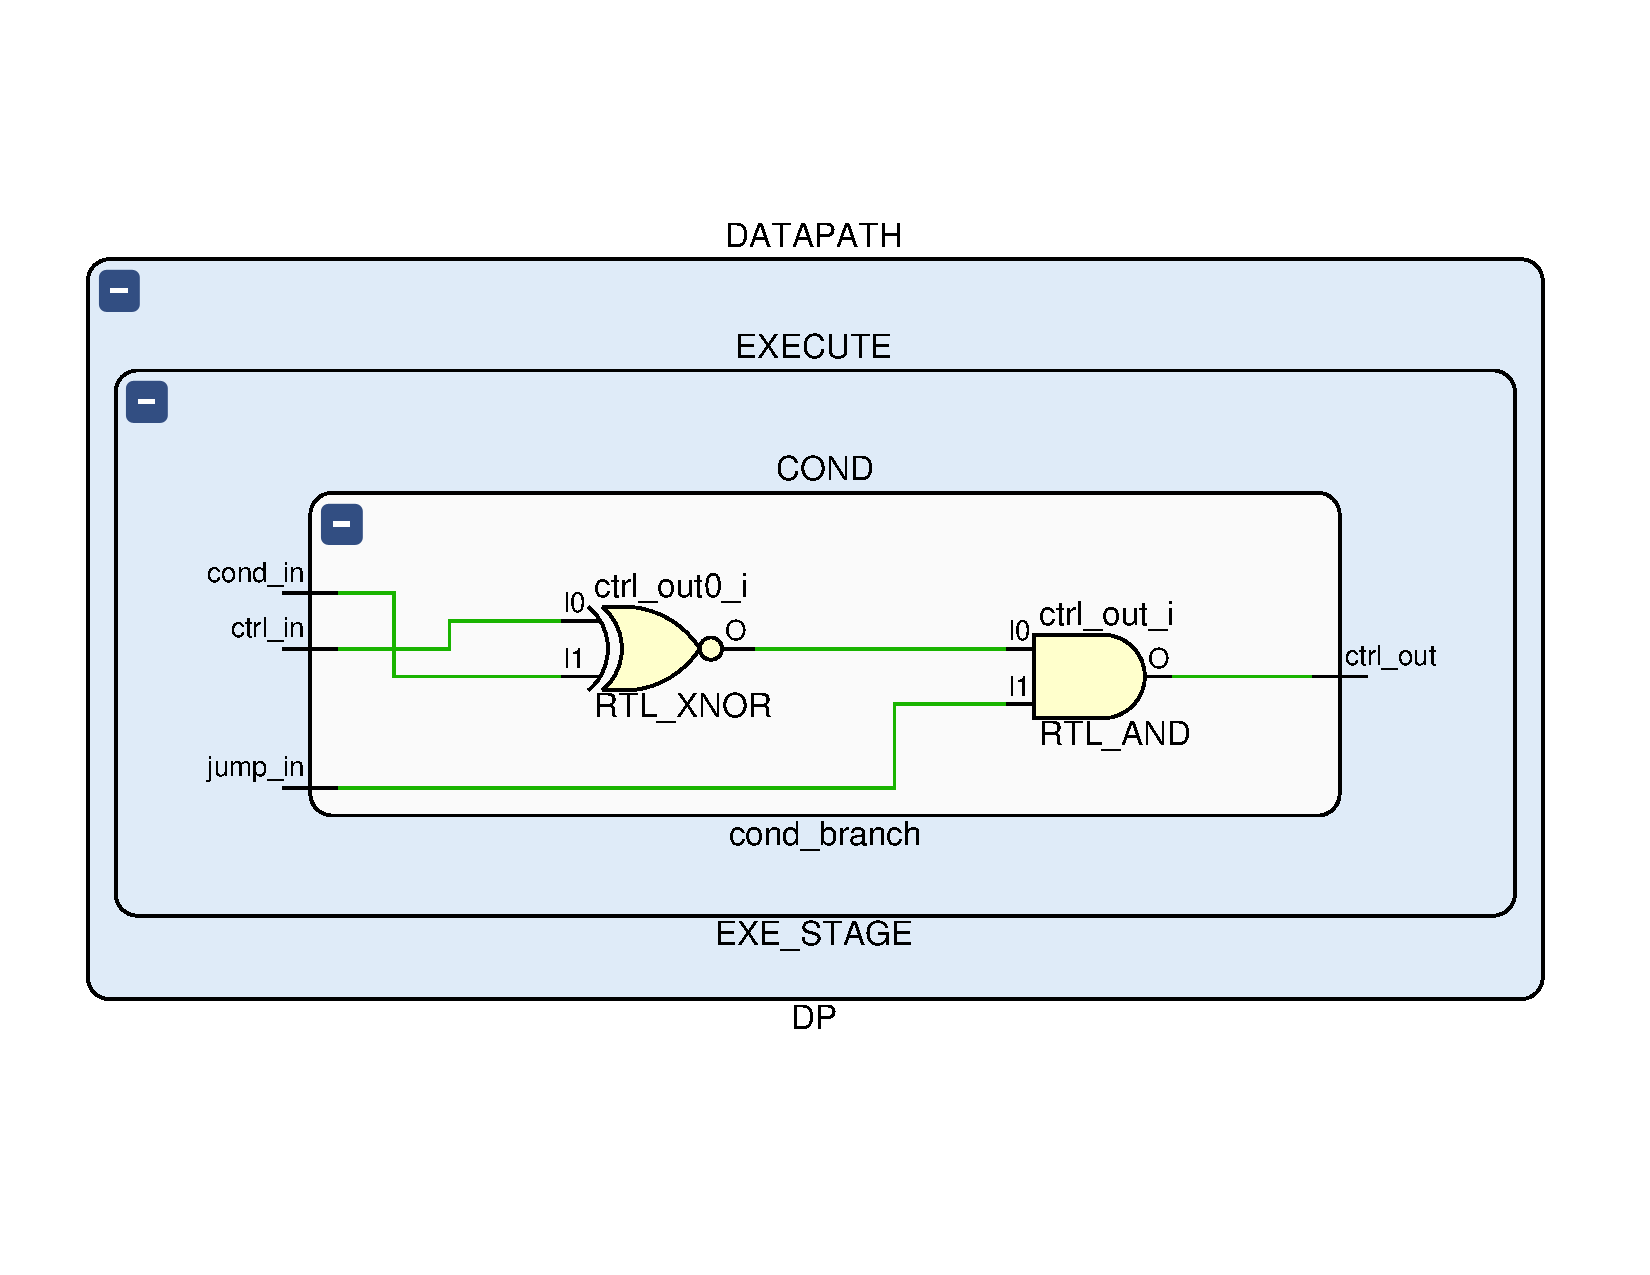
\includegraphics[width=\textwidth]{./chapters/figures/cond_branch.pdf} 
\caption{Schematic of \texttt{cond\_branch}.}
\end{figure}

\subsection{\texttt{cpsr}}
The Current Program Status Register was inspired by ARM architectures and contains the four main condition code flags generated by any given mathematical operation:
\label{cpsr}
\begin{itemize}
    \item \textbf{N} — Negative
    \item \textbf{Z} — Zero
    \item \textbf{C} — Carry
    \item \textbf{V} — Overflow.
\end{itemize}

Its outputs only reach the Datapath level, dying off before reaching the actual I/O of the microprocessor itself: as a matter of fact, they are intended for internal use only, and possibly provide an additional tool for implementing new \emph{conditional} instructions. They are left unused in the current state of this project.

\begin{figure}[!ht]
\centering
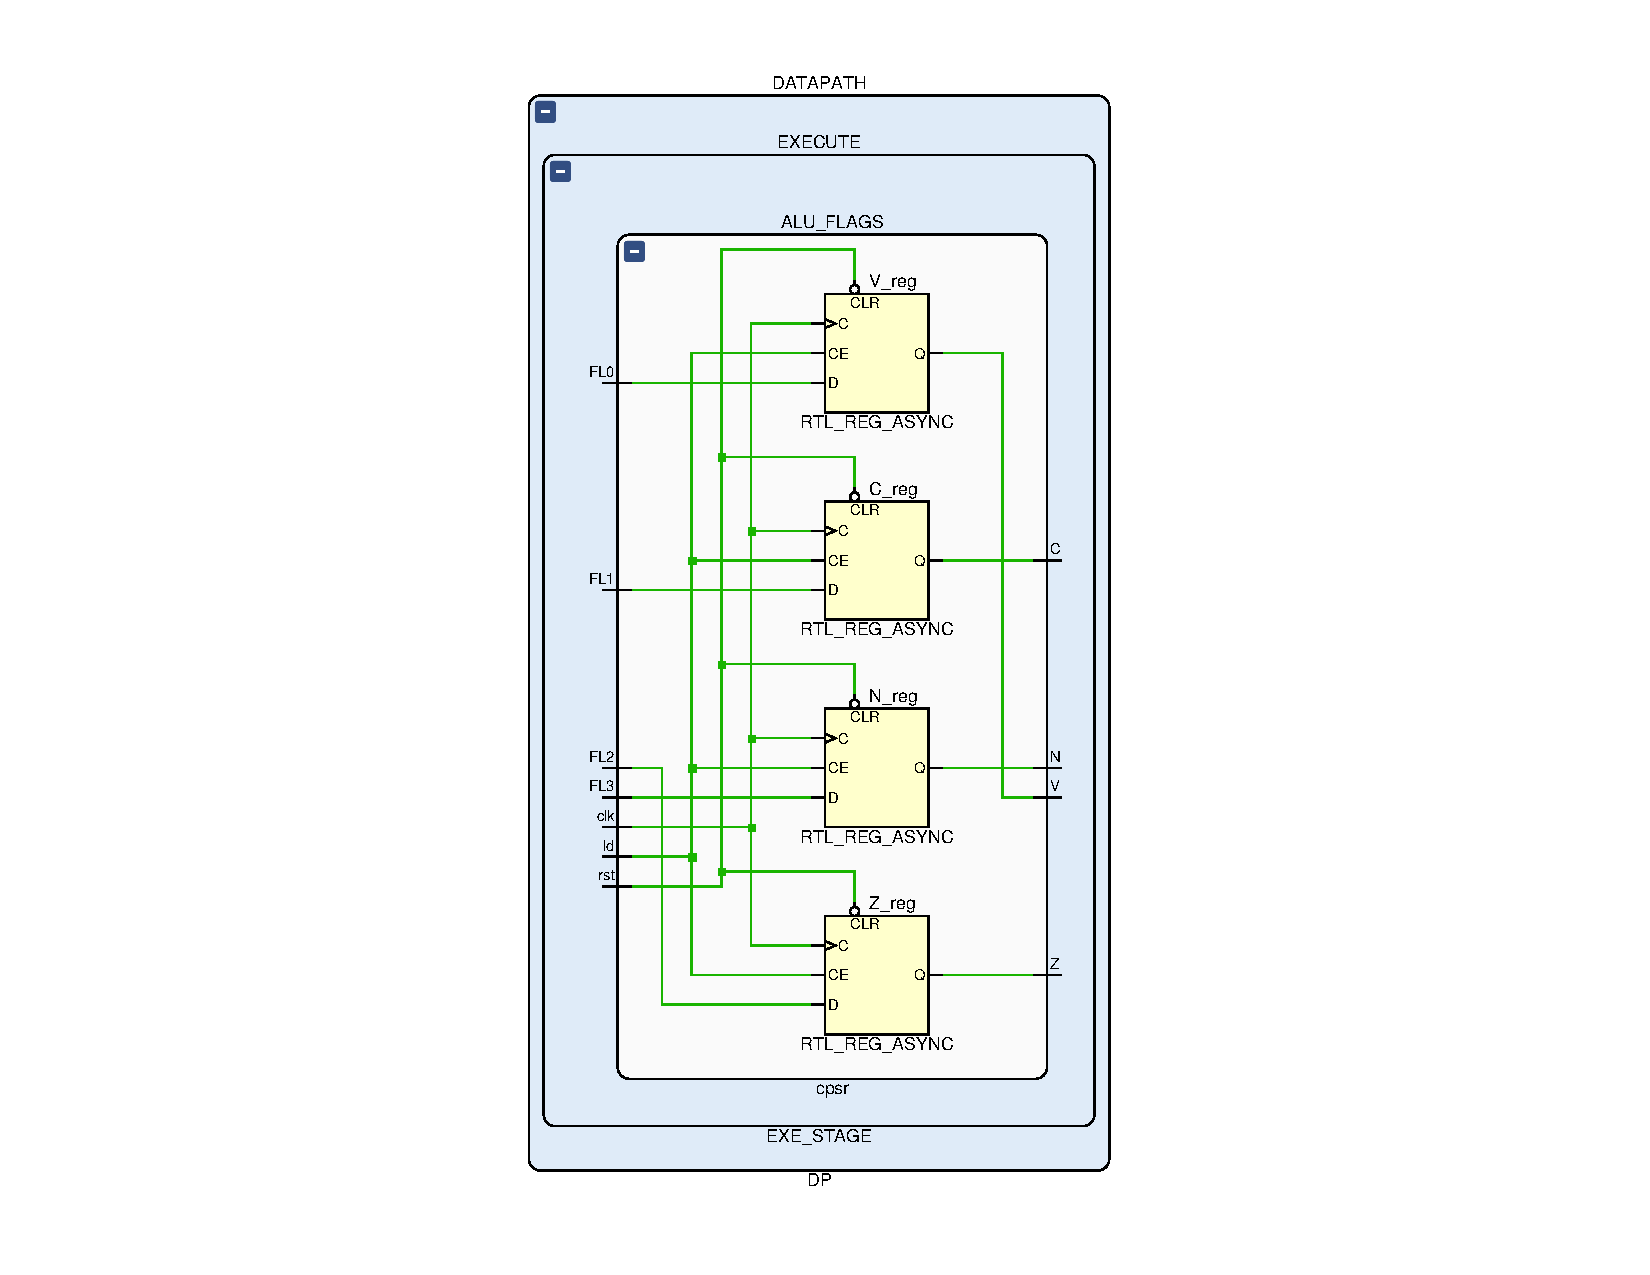
\includegraphics[width=\textwidth]{./chapters/figures/cpsr.pdf} 
\caption{Schematic of the \texttt{cpsr}.}
\end{figure}

\subsection{\texttt{gen\_mux21}}
\label{2to1}
A dataflow description of the classic \textbf{2 to 1} multiplexer with variable-width operands.

\begin{figure}[!ht]
\centering
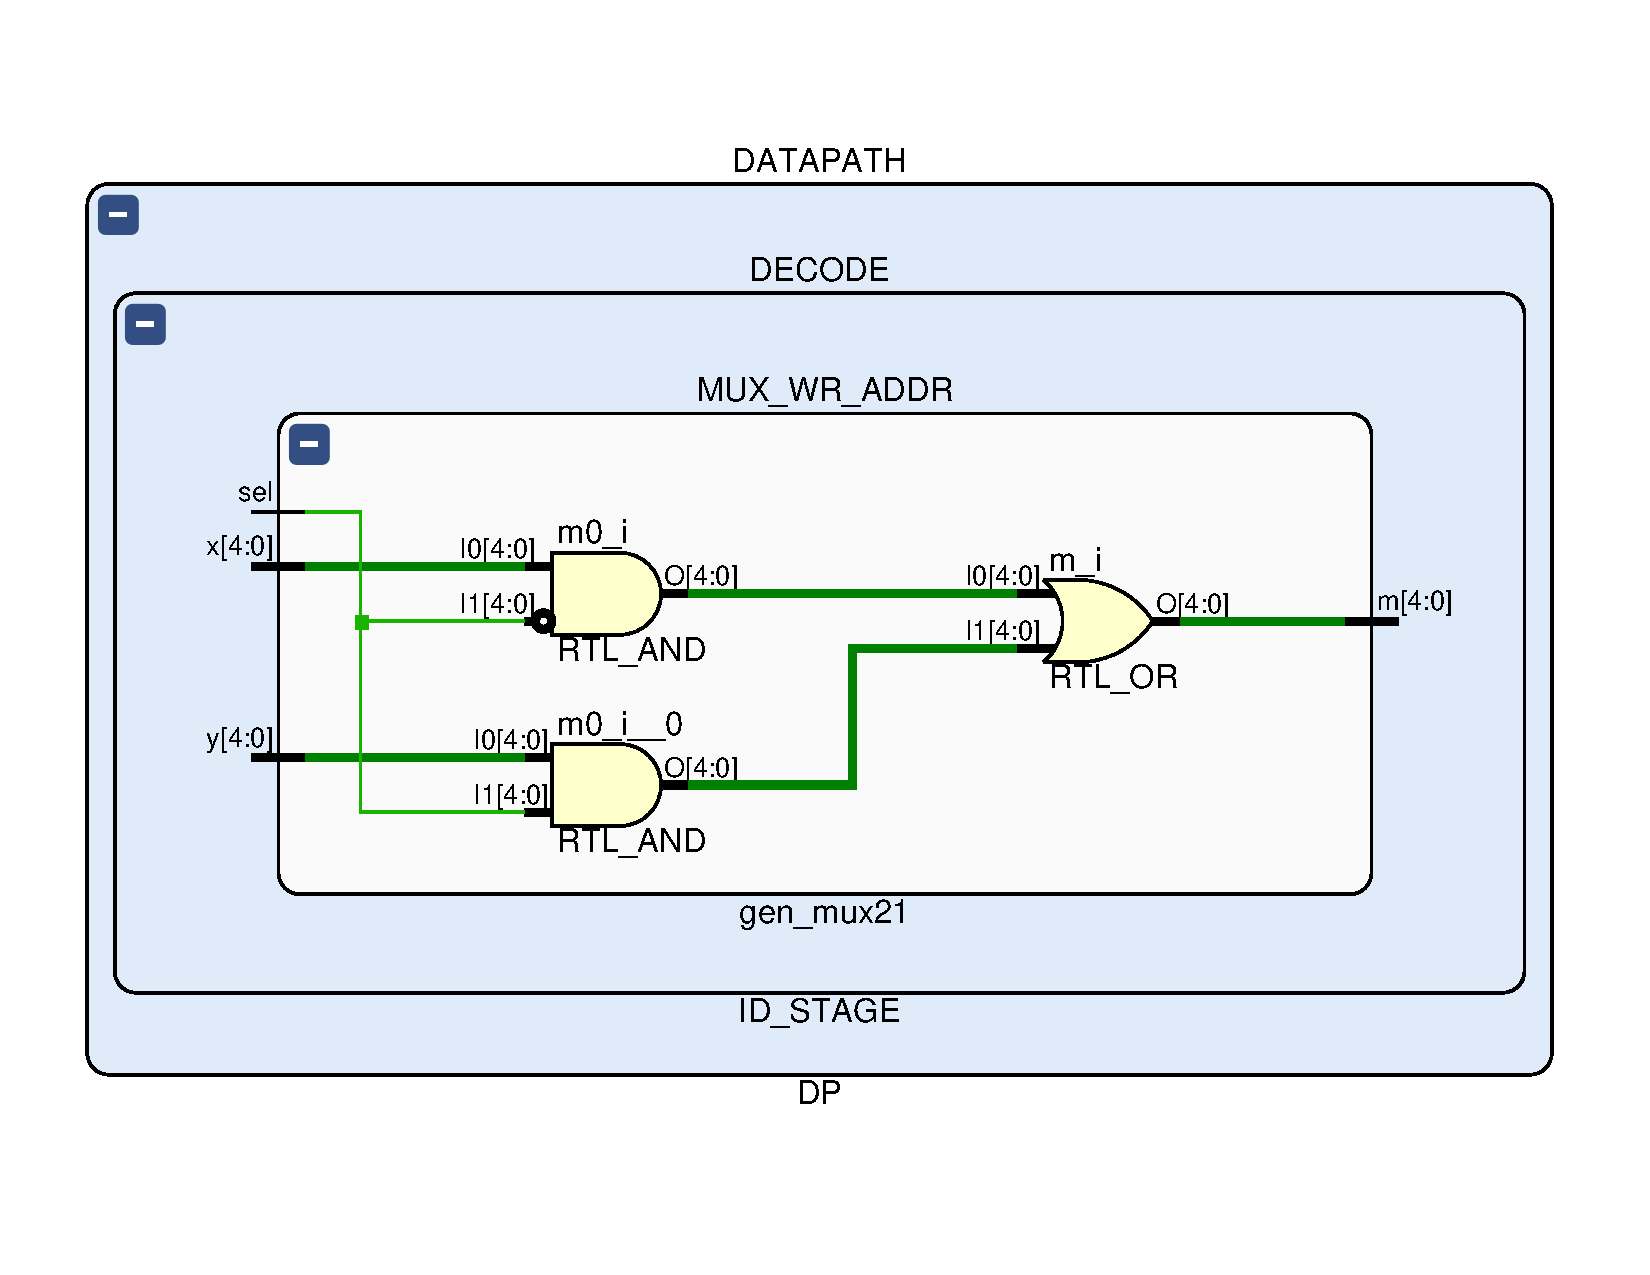
\includegraphics[width=\textwidth]{./chapters/figures/gen_mux21.pdf} 
\caption{Schematic of a \texttt{gen\_mux21}.}
\end{figure}

\subsection{\texttt{gen\_mux41}}
\label{4to1}
A slightly more complex revision of the above component, this \textbf{4 to 1} multiplexer requires a considerably larger amount of logic gates with two selectors to drive them. In the current state of the Datapath, its last two inputs (``10'' and `11'') are short-circuited, making the second selection bit a ``don't care'' whenever the first one is set to `1'.

\begin{figure}[!ht]
\centering
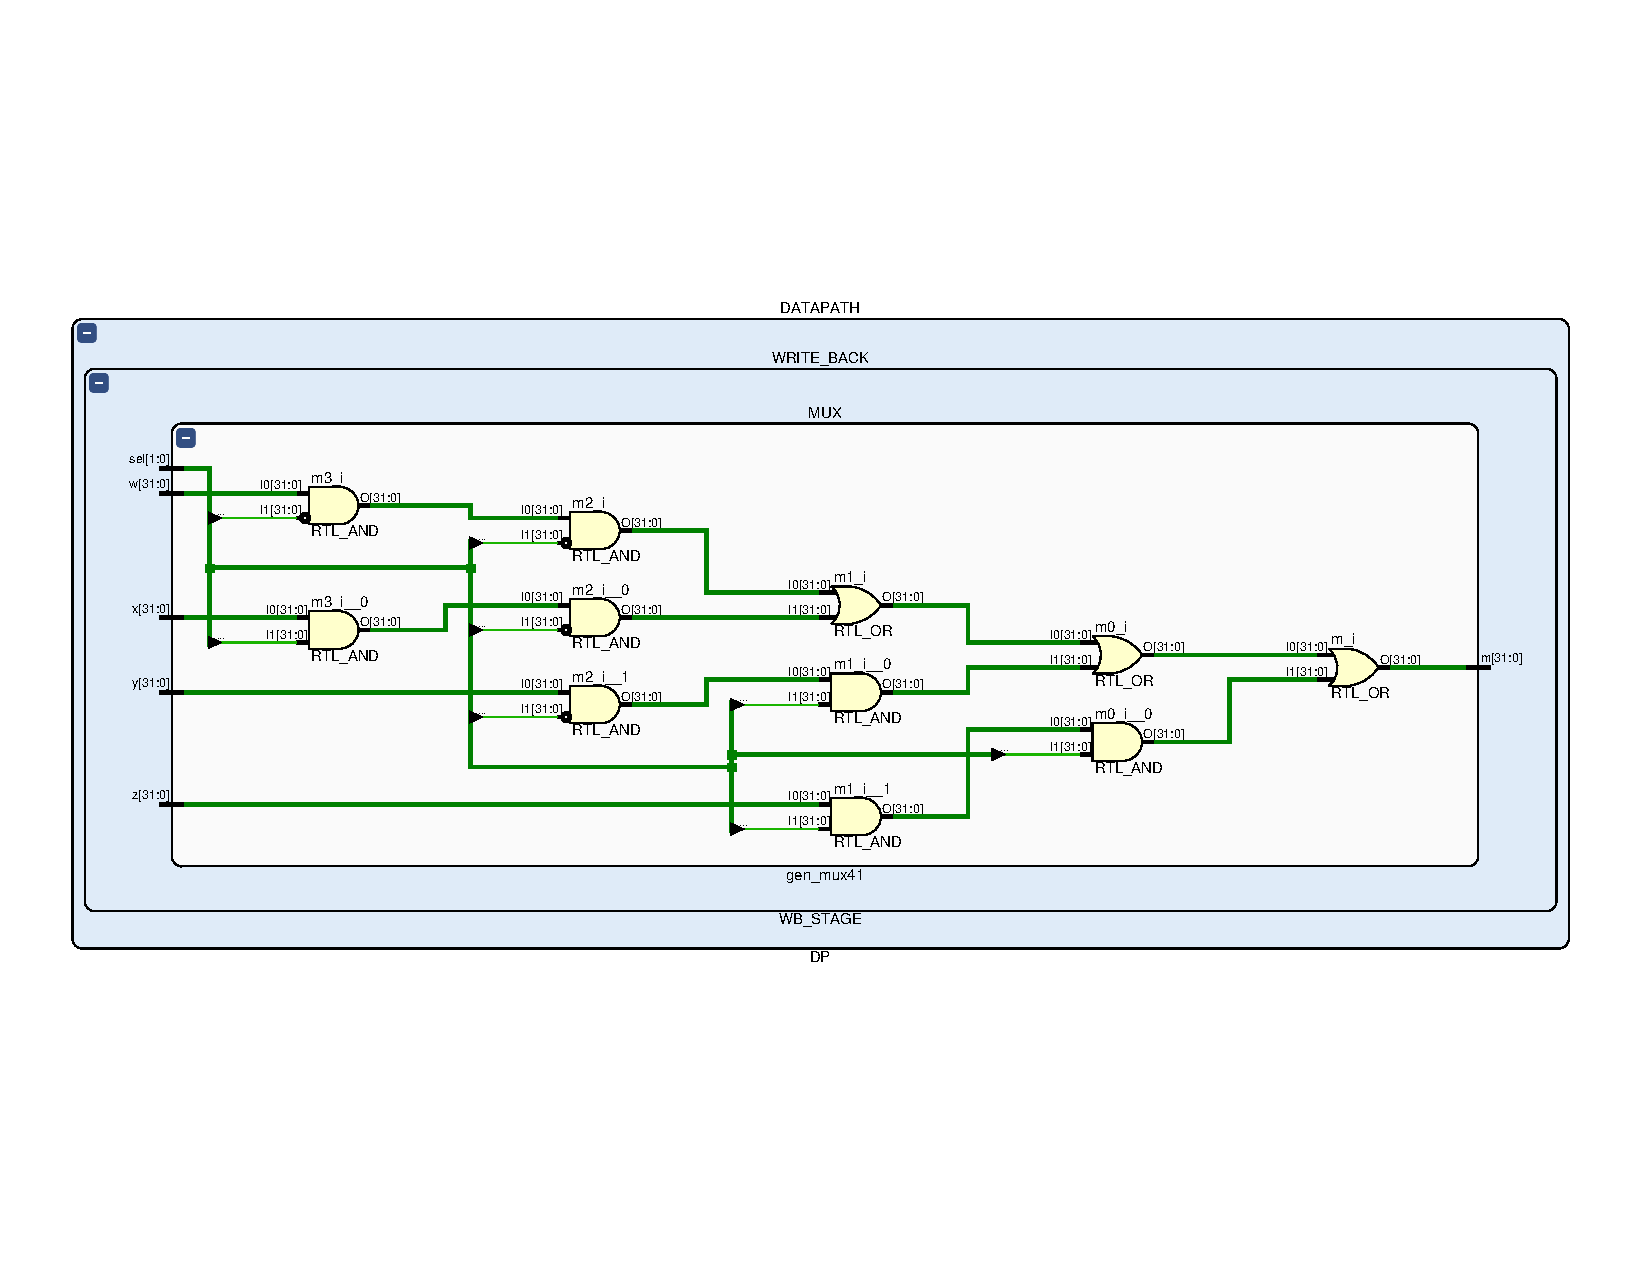
\includegraphics[width=\textwidth]{./chapters/figures/gen_mux41.pdf} 
\caption{Schematic of a \texttt{gen\_mux41}.}
\end{figure}

\subsection{\texttt{gen\_reg}}
A behavioral implementation of a variable-width register, sensitive to the rising edge of a clock signal, including an asynchronous reset and separate loading capabilities.

\begin{figure}[!ht]
\centering
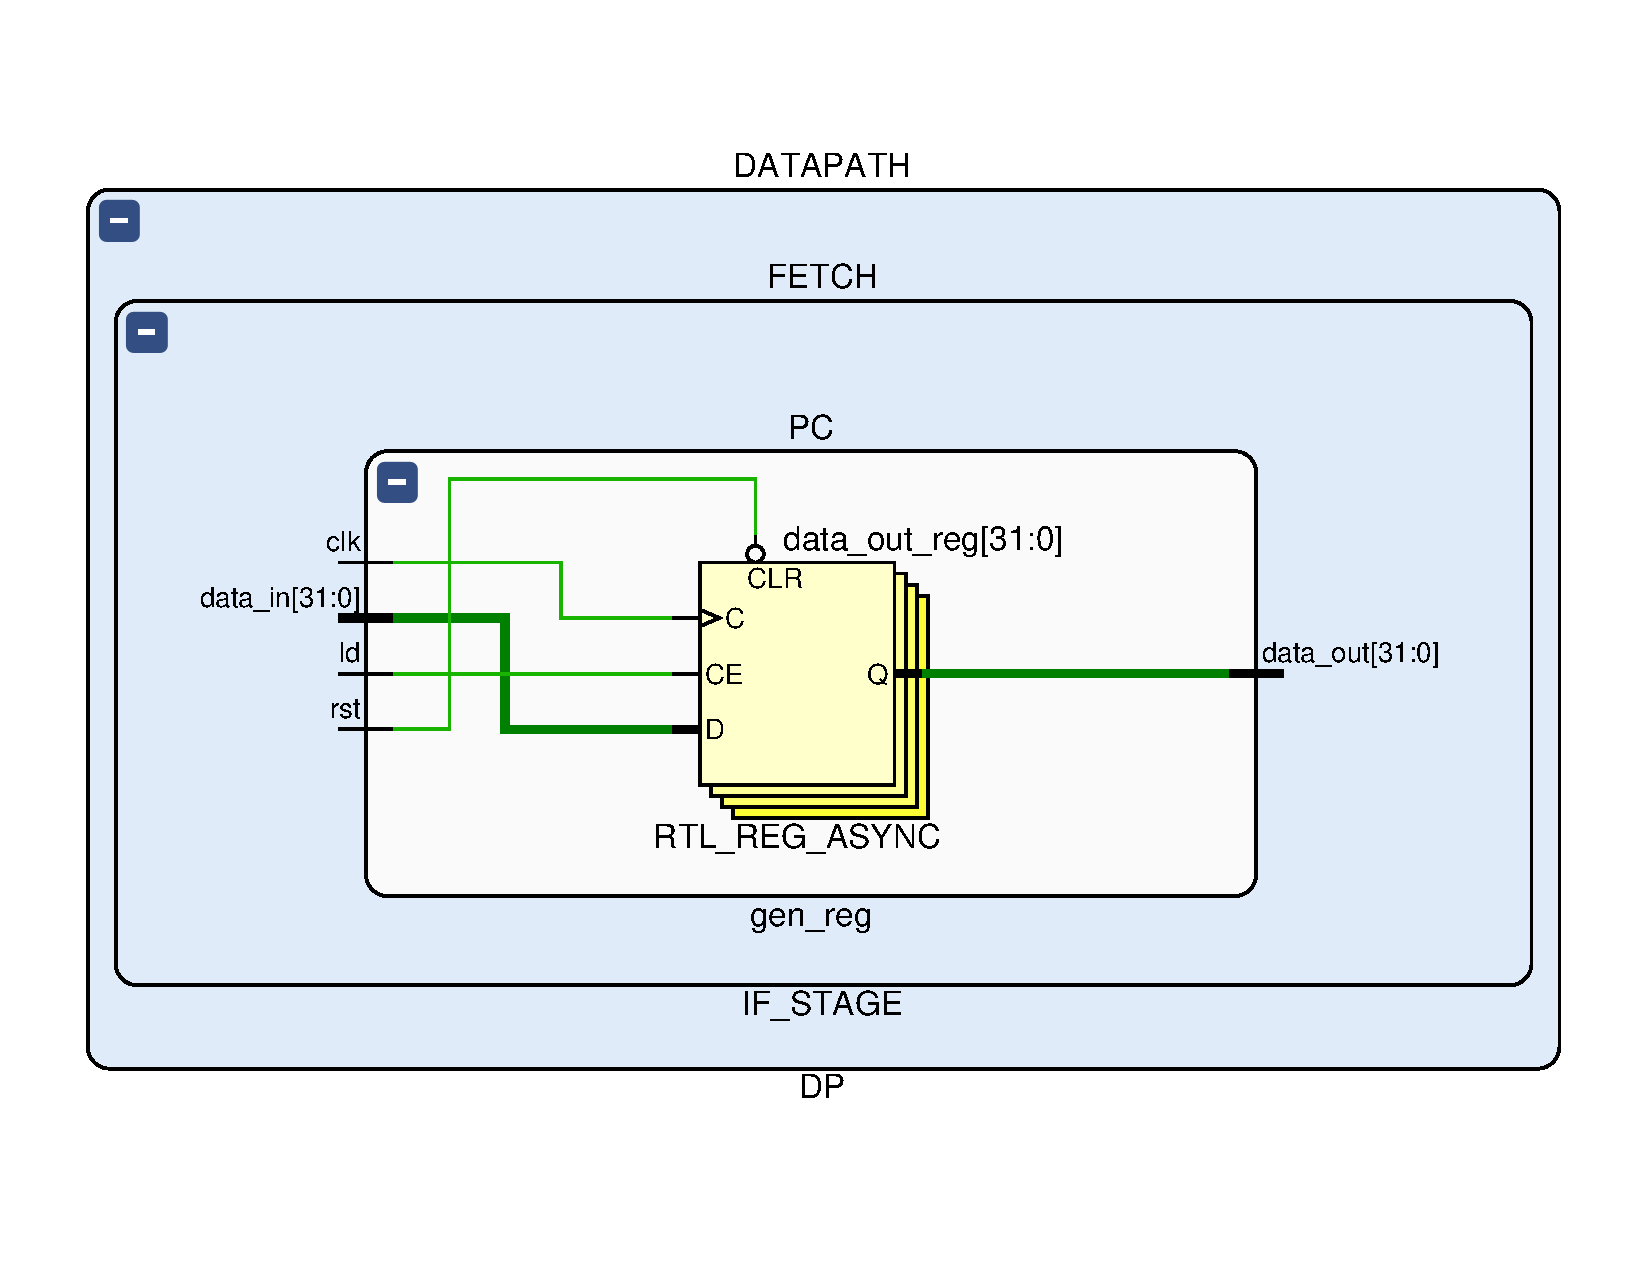
\includegraphics[width=\textwidth]{./chapters/figures/gen_reg.pdf} 
\caption{Schematic of a \texttt{gen\_reg}.}
\end{figure}

\subsection{\texttt{pc\_add}}
A behavioral adder used to compute the Next Program Counter with a fixed offset—the second operand is a constant equal to 4 in this context. Computation is \textbf{signed} in order to include backward jumps as well.

\begin{figure}[!ht]
\centering
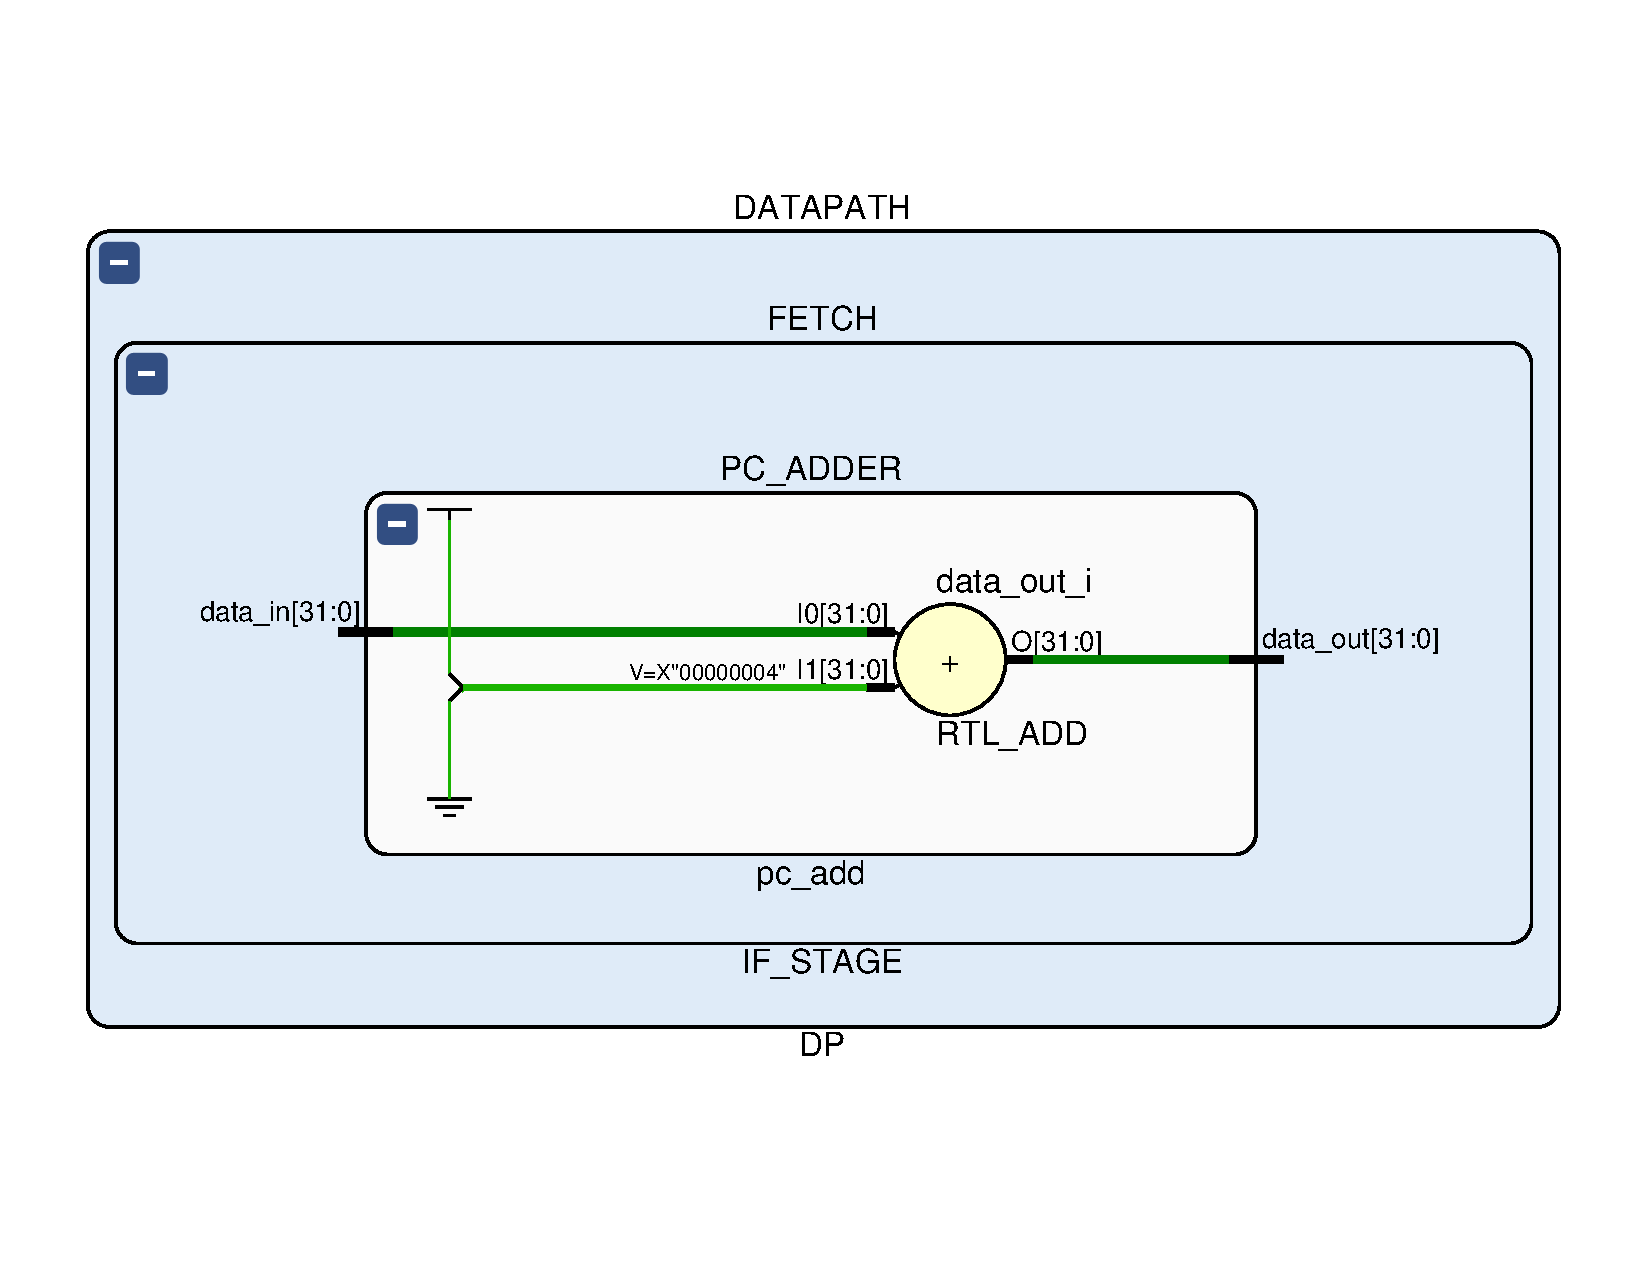
\includegraphics[width=\textwidth]{./chapters/figures/pc_add.pdf} 
\caption{Schematic of \texttt{pc\_add}.}
\end{figure}

\subsection{\texttt{reg\_file}}
This set of registers consists in a straightforward process that manages an internal memory, which is properly structured and accessed in compliance with the needs of the given ISA. Register \texttt{r0} is read-only, and set to an all-zero value during reset (asynchronous) in a pure MIPS-like fashion.

One interesting characteristic is the direct bypass of the internal signals in case of simultaneous reading and writing operations on the same address: the corresponding location will of course take on the provided value, but the latter will immediately be forwarded to the output port instead of still being gathered from that same cell. This mechanism was implemented in an effort to avoid causing undefined or unstable events during concurrent operations on the same register, providing an even faster solution to such issue in terms of delay.

\begin{figure}[!ht]
\centering
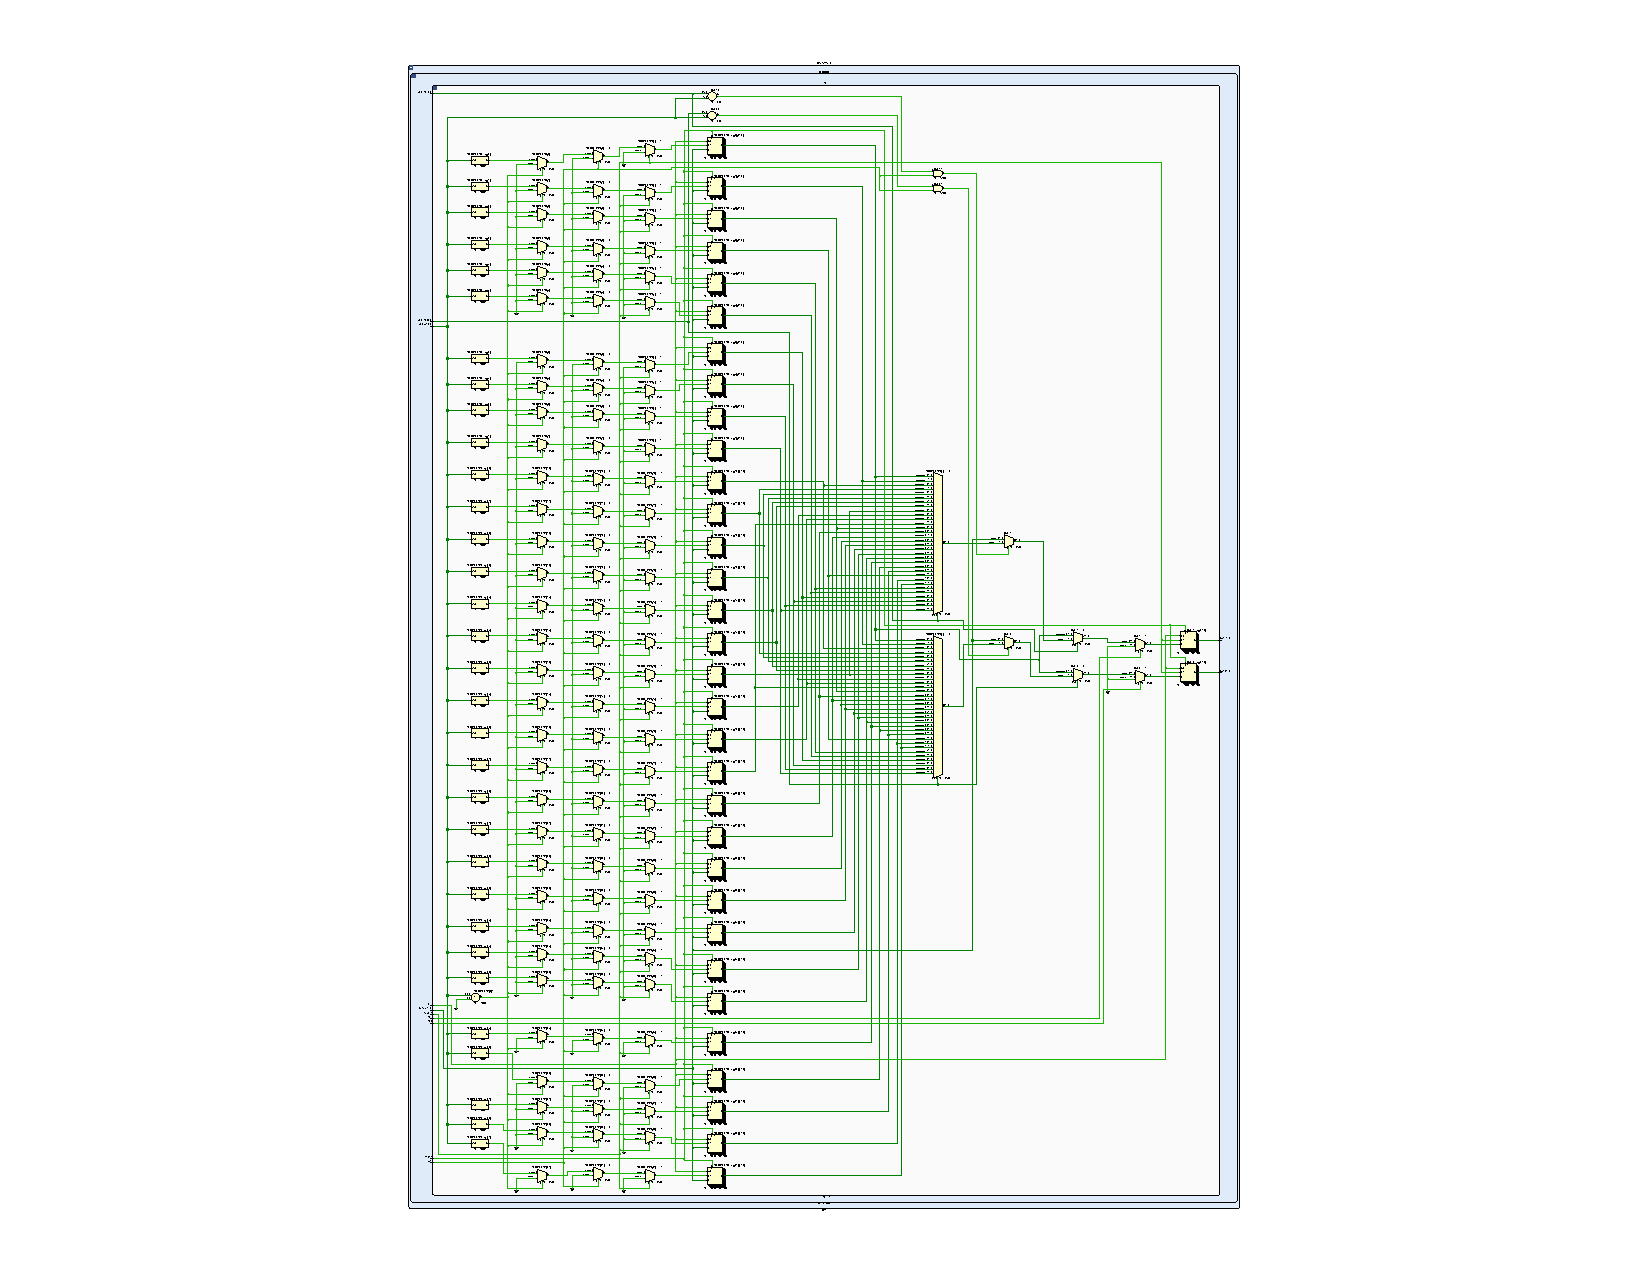
\includegraphics[width=\textwidth]{./chapters/figures/reg_file.pdf} 
\caption{Schematic of the \texttt{reg\_file}.}
\end{figure}

\subsection{\texttt{sign\_ext\_alt}}
\label{alternate}
An alternate, more complex version of the subsequent component that provides sign extension and zero padding capabilities. This is a highly specialized block that is only used inside the Memory pipeline stage, and the performed operations are as follows:
\begin{table}[!ht]
\centering
\begin{tabular}{cc|c}
\toprule
\texttt{ctrl\_in} & \texttt{zero\_padding} & Action\\
\midrule
0 & 0 & Extend byte sign\\
0 & 1 & Zero pad byte\\
1 & 0 & Extend half-word sign\\
1 & 1 & Extend actual sign\\
\bottomrule
\end{tabular}
\end{table}

\begin{figure}[!ht]
\centering
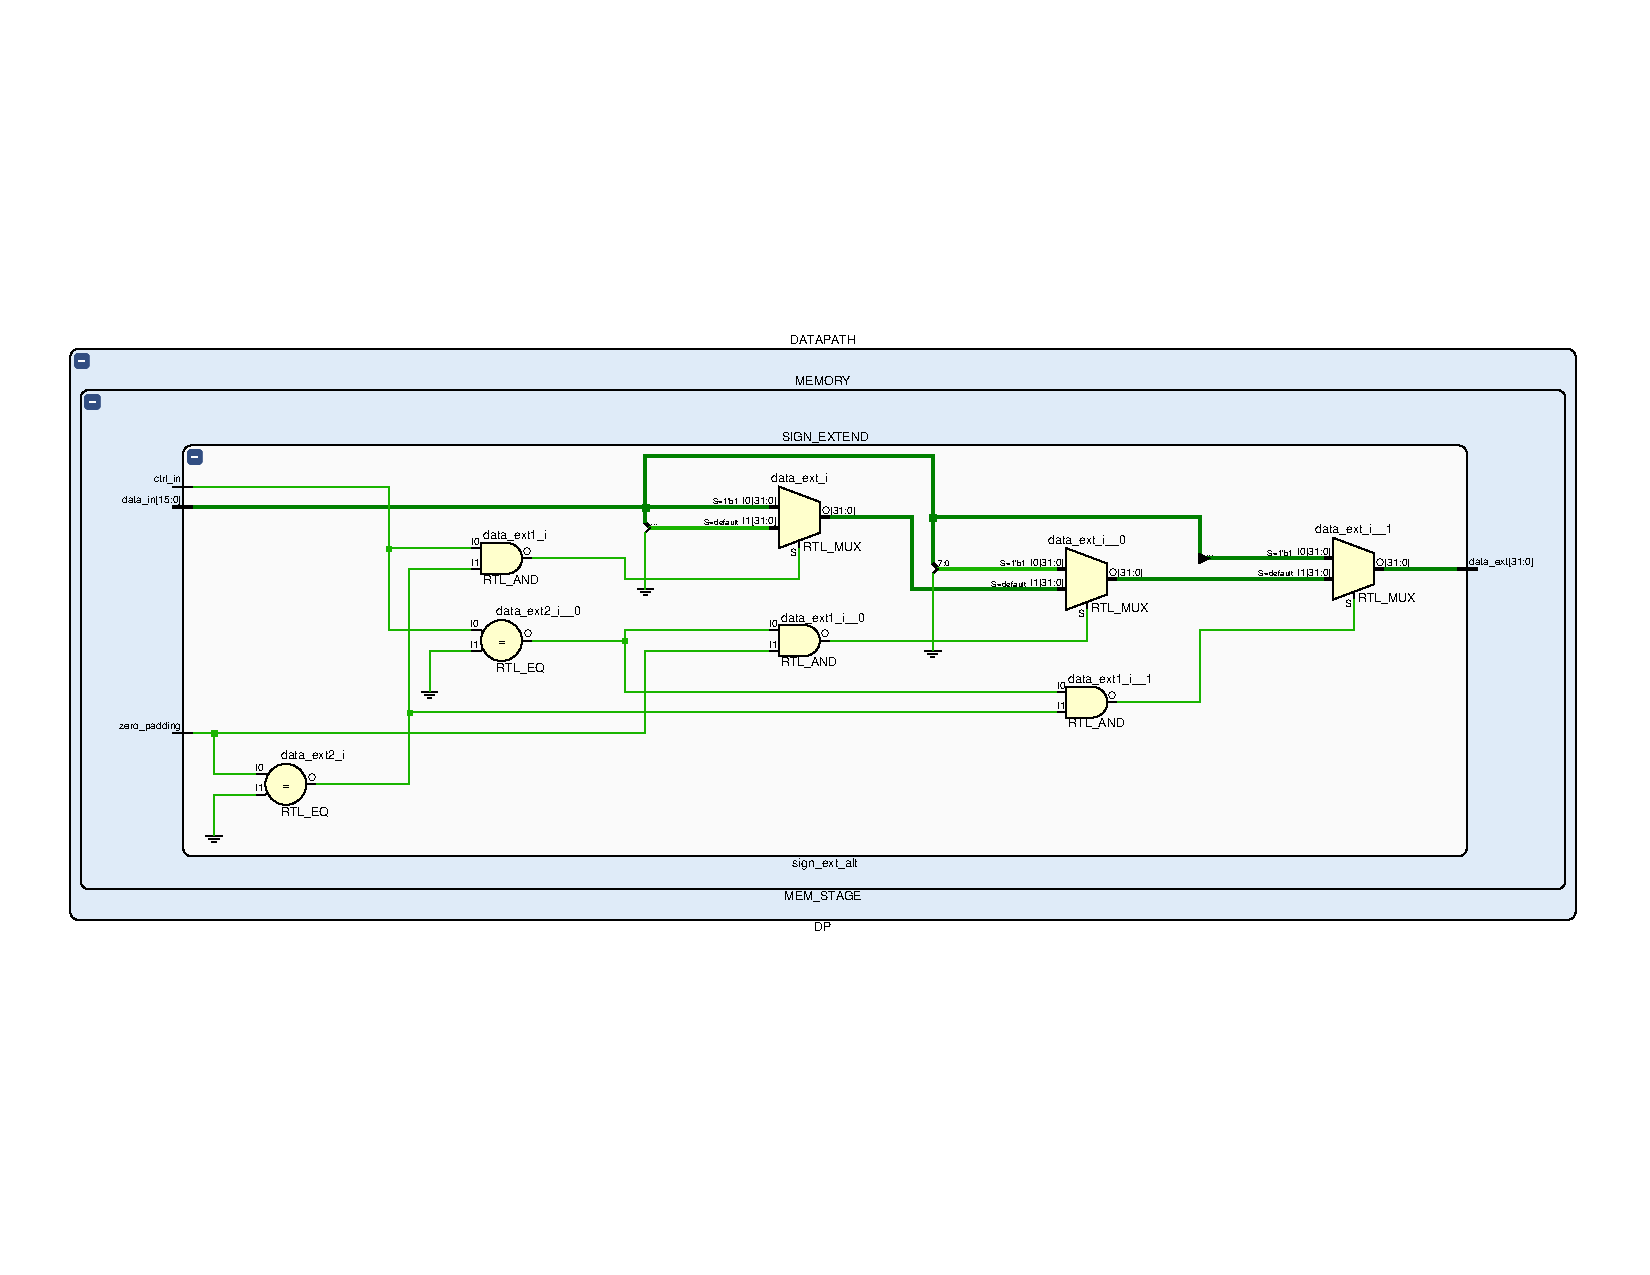
\includegraphics[width=\textwidth]{./chapters/figures/sign_ext_alt.pdf} 
\caption{Schematic of \texttt{sign\_ext\_alt}.}
\end{figure}

\subsection{\texttt{sign\_ext}}
This is a simplified version of the previous block, used inside the Decode stage this time. The implemented functionalities are again quite specific:
\begin{table}[!ht]
\centering
\begin{tabular}{cc|c}
\toprule
\texttt{ctrl\_in} & \texttt{zero\_padding} & Action\\
\midrule
0 & - & Extend actual sign\\
1 & 0 & Extend internal sign\\
1 & 1 & Zero pad actual length\\
\bottomrule
\end{tabular}
\end{table}

\begin{figure}[!ht]
\centering
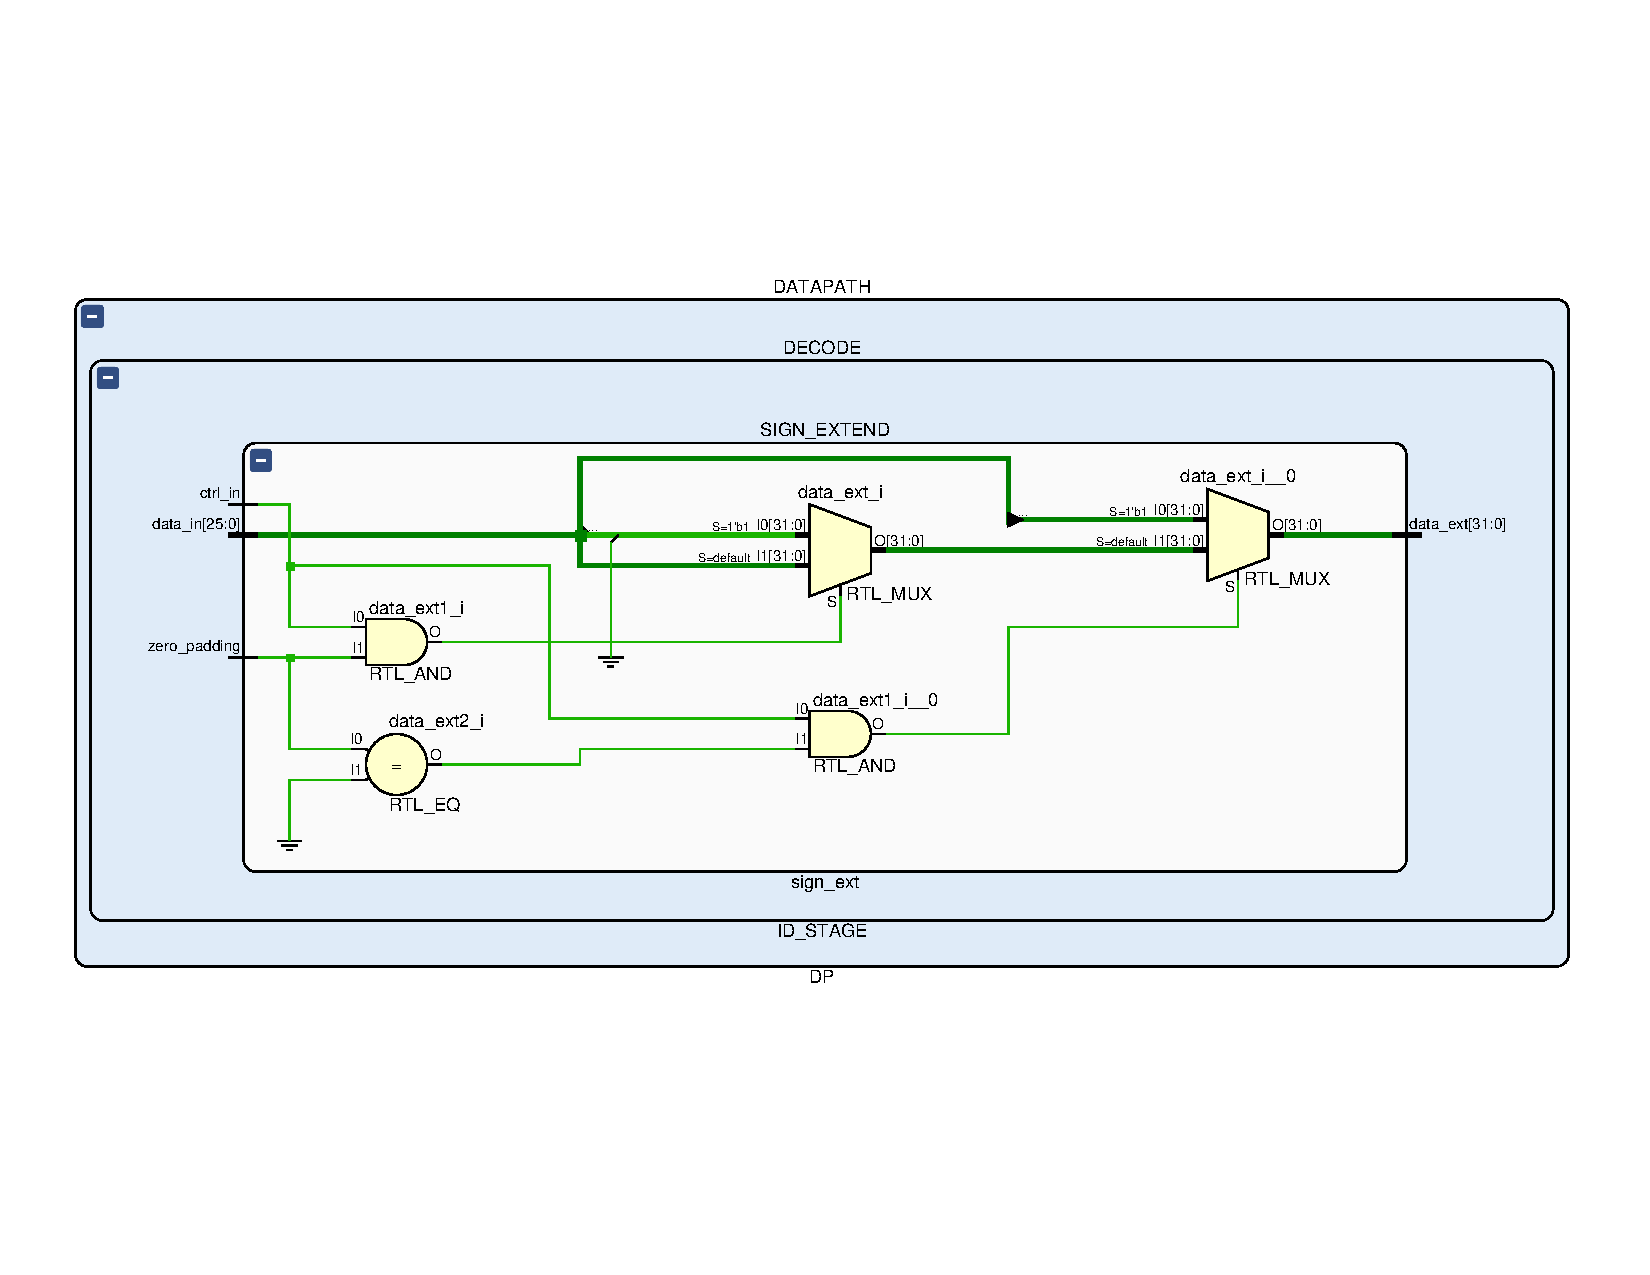
\includegraphics[width=\textwidth]{./chapters/figures/sign_ext.pdf} 
\caption{Schematic of \texttt{sign\_ext}.}
\end{figure}

\subsection{\texttt{zero\_check}}
A trivial combinational unit aimed at recognizing whenever its variable-width input vector is made of only zeros, used in conjunction with \nameref{cond-branch} to generate the selector (subsequently made synchronous) of the multiplexer responsible for branches.

\begin{figure}[!ht]
\centering
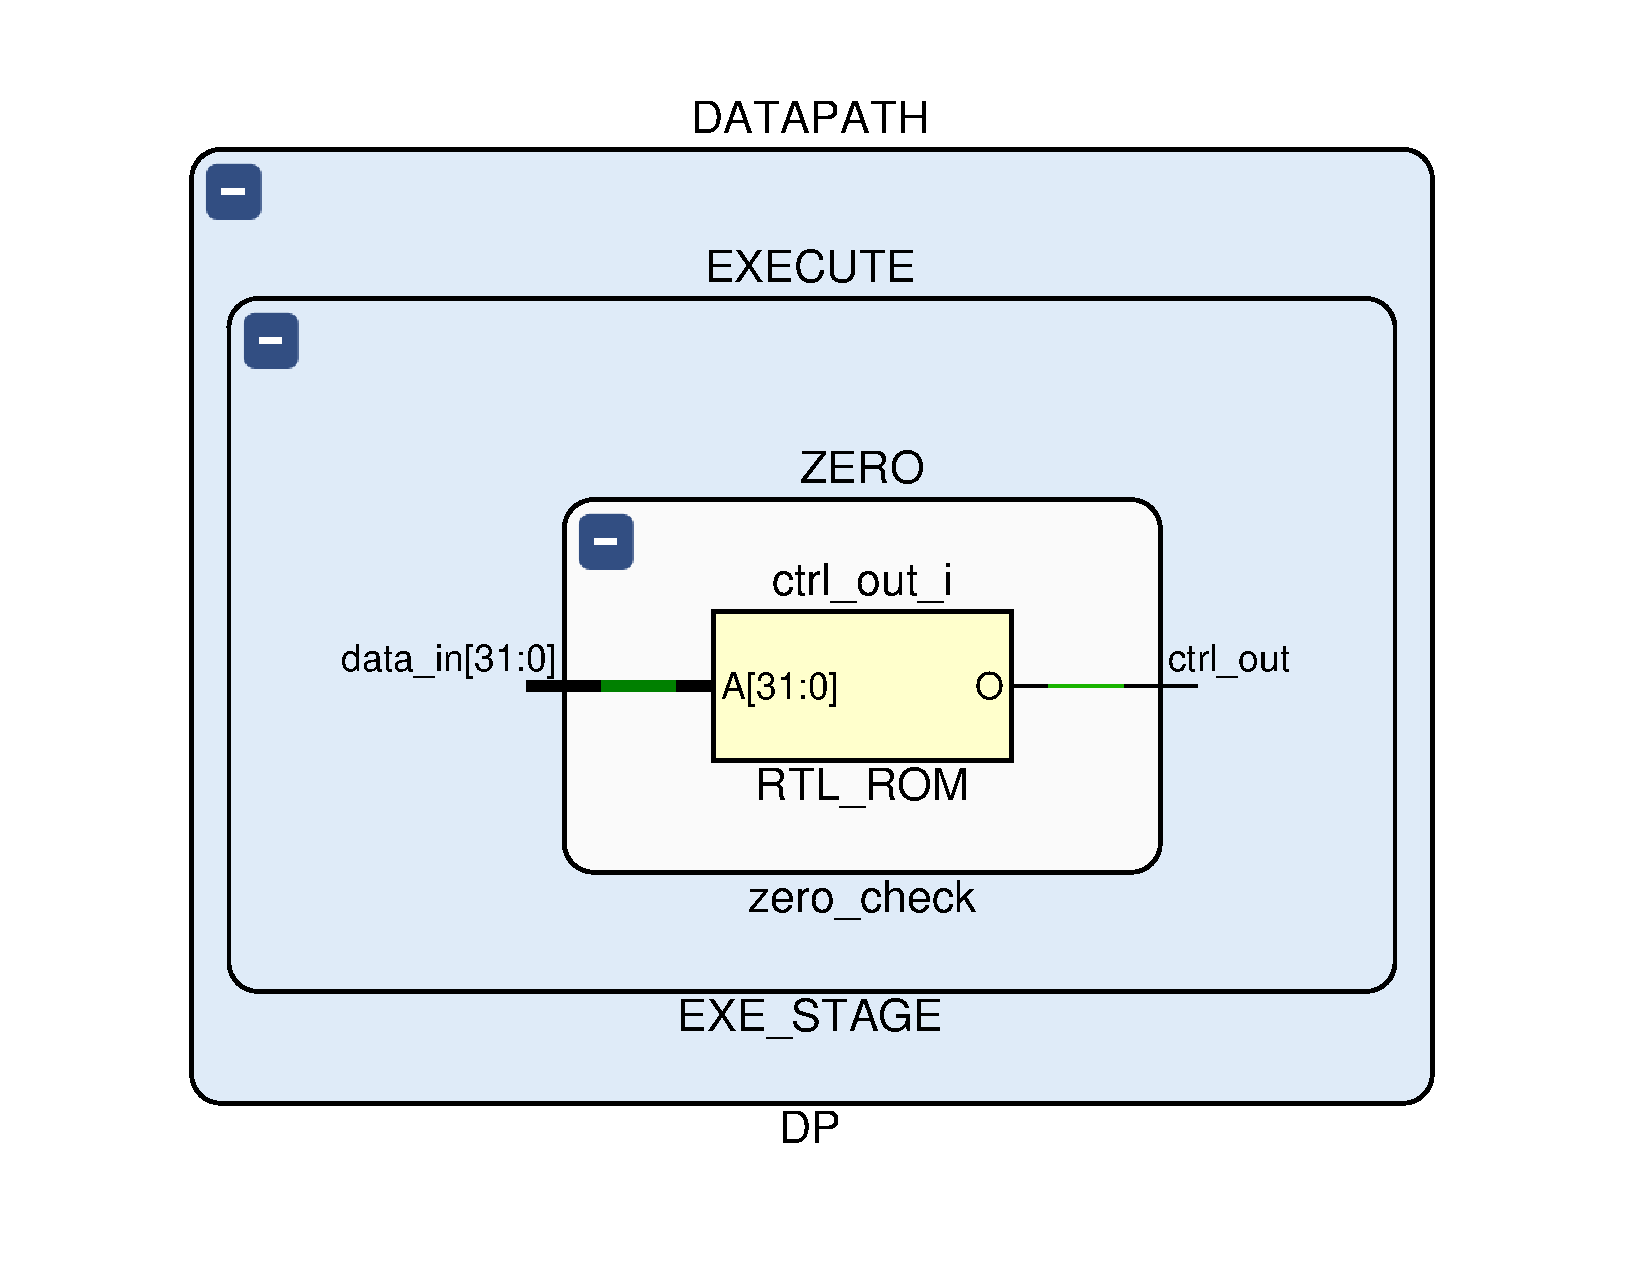
\includegraphics[width=\textwidth]{./chapters/figures/zero_check.pdf} 
\caption{Schematic of \texttt{zero\_check}.}
\end{figure}

\section{Pipeline stages}
These five macro-structures represent the main building blocks of the Datapath, with the purpose of combining and linking all the previously described low-level components in order to create a unique and coherent unit. The latter would have to perform any given functionality during the span of five clock cycles, making timing synchronization of paramount importance.

Because of this last aspect, these mid-level stages are here listed following their temporal order inside the microprocessor pipeline.
\subsection{\texttt{IF}}
A very straightforward structural architecture that includes the interface with the external Instruction Memory. It generates the address to the next operation that will be fed to the whole pipeline, whilst also taking in the current one that needs to be tackled with.

An array of synchronization registers had to be included in the path related to the Next Program Counter as to align it the one related to actual instructions instead (this concept will become clearer during the explanation of the \nameref{top-level} layer). This will obviously cause an initial delay between the arrival time of every command and its actual execution, but the timing interval between subsequent ones will still comply to the \textbf{5-cycle} pipeline of choice.

\subsection{\texttt{ID}}
A collection of blocks that are needed to store the actual data that travels throughout the whole design in a very fast internal location. Many synchronization registers are included, while the first sign extension block performs the required operation on the Immediate field depending on the type of instruction that is being analyzed.

One multiplexer is dedicated to selecting the correct field of R-Type versus I-Type instructions that would indicate the destination register RD. Moreover, a simple OR port in front of the writing address of the register file was introduced to easily place the NPC inside \texttt{r31} during ``Jump and Link'' operations (as per specifications).

\subsection{\texttt{EXE}}
The core of computation of the DLX microprocessor, it works on integer values only. Two multiplexers select the correct operands to be sent to the ALU, while a pair of combinational blocks generates the correct control signals during branch evaluations.

A noticeable amount of synchronization register are instantiated alongside the register dedicated to storing the status flags computed by the same ALU. The latter has, in turn, a dedicated internal signal aimed at selecting the correct operation to perform during the execution of any given instruction.

\subsection{\texttt{MEM}}
This stage contains another external interface, this time with the external Data Memory. It is in fact capable of providing both addresses and data to the input ports of such peripheral block, whilst directly forwarding the required control signals to the same from the Control Unit itself.

Read values are instead selected by means of an output multiplexer, after possibly going through the alternate sign extension module, which is used whenever a value shorter than 32-bits has to be loaded. A second multiplexer picks the correct Program Counter that needs to be sent to the Instruction Fetch stage.

\subsection{\texttt{WB}}
The simplest among all the pipeline stages, its only purpose is that of selecting the correct outcome that needs to be sent to the Register File. The \texttt{IR} signal goes through this stage untouched, while the 4-input multiplexer can only actually pick between three different alternatives:
\begin{table}[!ht]
\centering
\begin{tabular}{cc|c}
\toprule
\texttt{JAL\_MUX\_SEL} & \texttt{WB\_MUX\_SEL} & Selection\\
\midrule
0 & 0 & ALU Output\\
0 & 1 & Memory Output\\
1 & - & Next Program Counter\\
\bottomrule
\end{tabular}
\end{table}

\section{Higher level entities}
Two main design units are eventually connected to each other in order to achieve the final architecture of the DLX microprocessor: in the following, the culminating blocks of the entire model are listed using a topological order.

\subsection{\texttt{DP}}
The Datapath of this design consists in nothing more than an extensive set of connections between the five aforementioned pipeline stages, with a multitude of internal signals aimed at creating a clean and direct interface between them.

This composite structure is also responsible for communicating with both external Memories, actually generating the required I/O that has to later be handled by the top-level entity.

\begin{figure}[!ht]
\centering
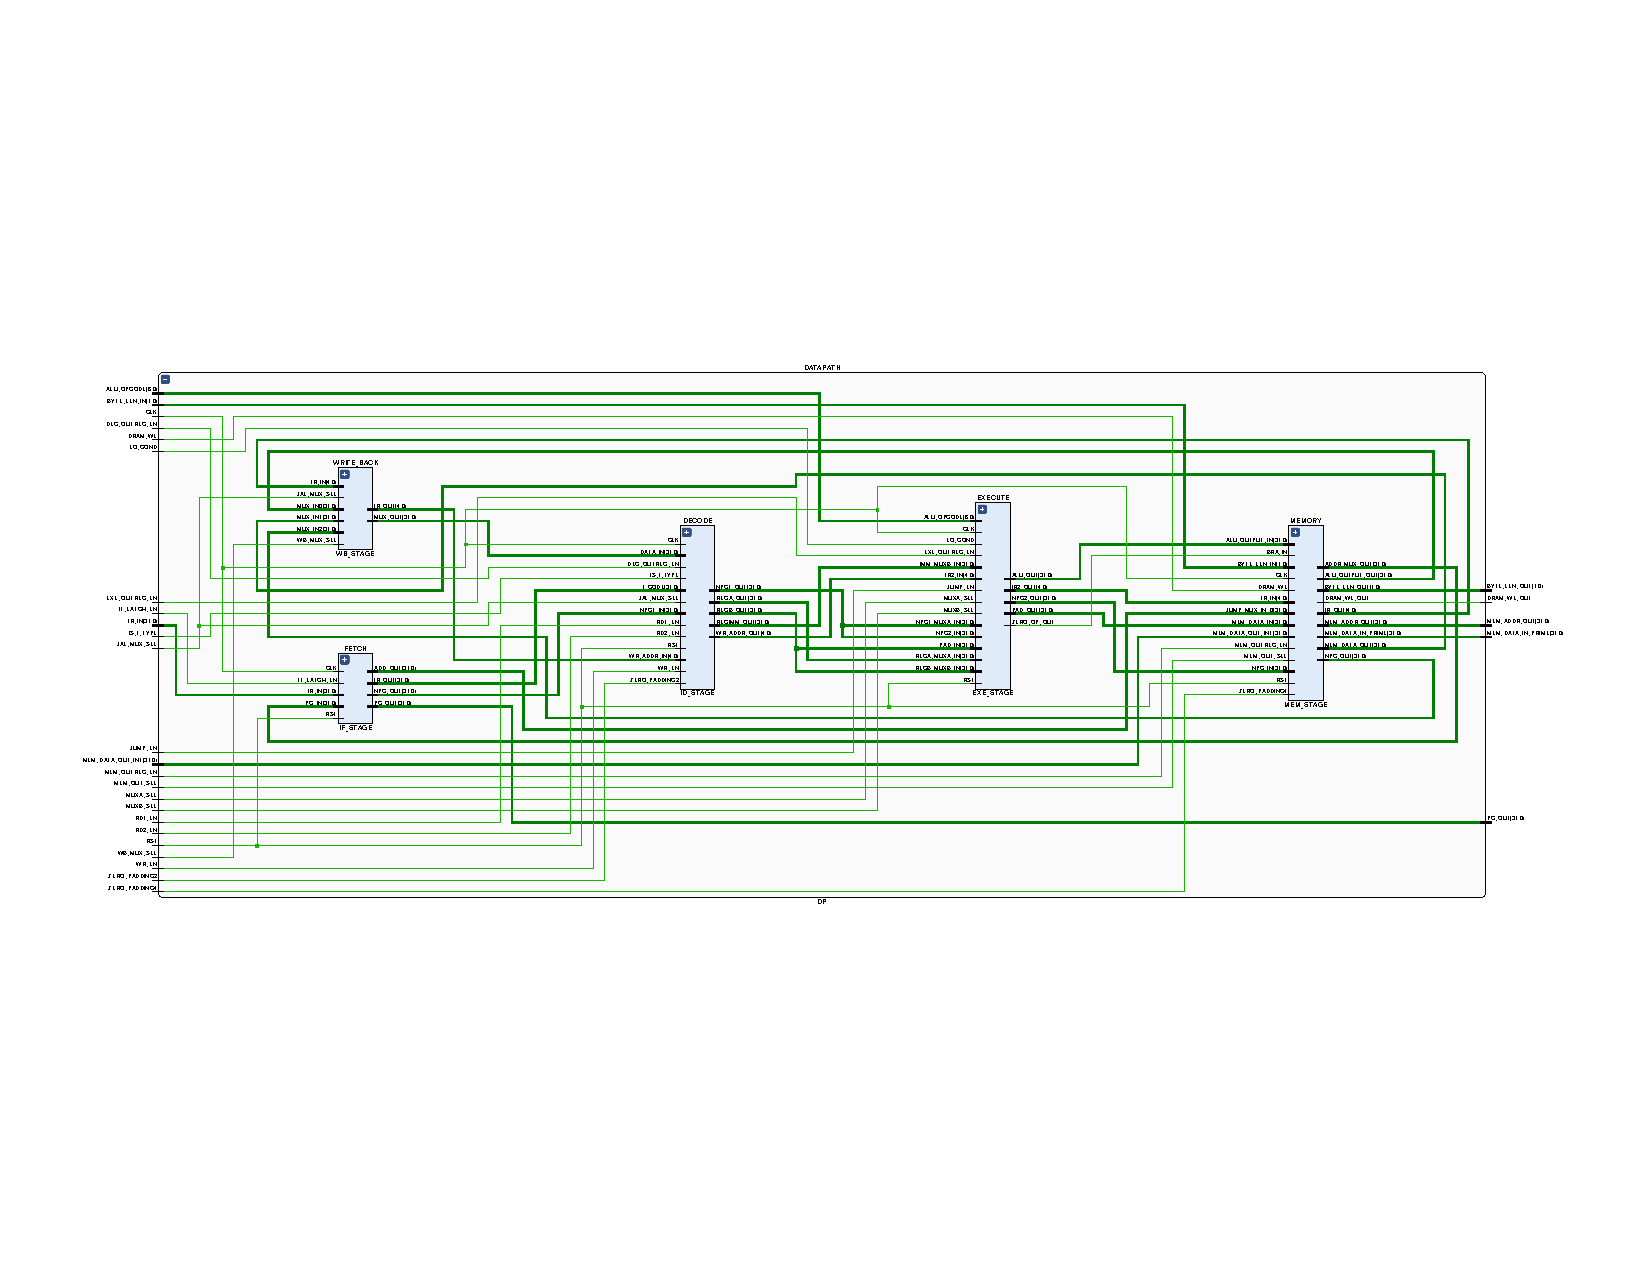
\includegraphics[width=\textwidth]{./chapters/figures/DP.pdf} 
\caption{High-level view of the \texttt{DP}.}
\end{figure}

\subsection{\texttt{CU\_HW}}
The Control Unit of this microprocessor is the module that actually manages the functionalities provided by the Datapath, feeding the latter with the correct combination of control bits at any given time. Its reset is still asynchronous, and it of course has to comply with the same 5-stage pipeline.

\label{control-unit}
The chosen approach for this structure was a \textbf{hardwired} implementation, in which the control word codings are contained inside an internal LUT (read-only memory element). Starting from the input instruction, this module has to parse the two fields of interest, i.e. OPCODE and FUNC, in order to select the corresponding operation, ultimately driving all the other components located inside the architecture. Messages directed to both the ALU and a possible FPU are taken care of by means of custom VHDL types and dedicated processes.

Control words are picked from a dictionary of known values thanks to their unique identifier (whose hexadecimal values were provided inside the official specifications) in such a way that the output assignment gets reduced to a few subsequent steps:
\begin{enumerate}
\item Parsing and identification of the information coming from the Instruction Memory
\item Search operation inside the internal LUT (with several ``holes'' representing invalid entries)
\item Pipelined output assignment and message generation for the execution unit(s).
\end{enumerate}

In case of an out-of-range request, or even a command that is yet to be implemented, this fault-tolerant architecture automatically returns a \emph{nop}.

\subsection{\texttt{DLX}}
This component sits at the highest level of abstraction of the whole design space, combining the contributions of both the previously described modules. It is the main block that would later be simulated, synthesized and taken through the required physical design process.

\label{top-level}
At this point, it's important to highlight the essential role of an additional synchronization register that needed to be inferred (indirectly, through a VHDL process) between the Instruction Memory and the Datapath inside this layer—the Control Unit must be exactly \textbf{one} clock cycle in advance with respect to the latter in order to issue the correct coding at the right time.

The port list of this structure contains the main I/O of the DLX itself, while the whole set of generics needed inside all the previously mentioned modules are grouped right at this level.

\begin{figure}[!ht]
\centering
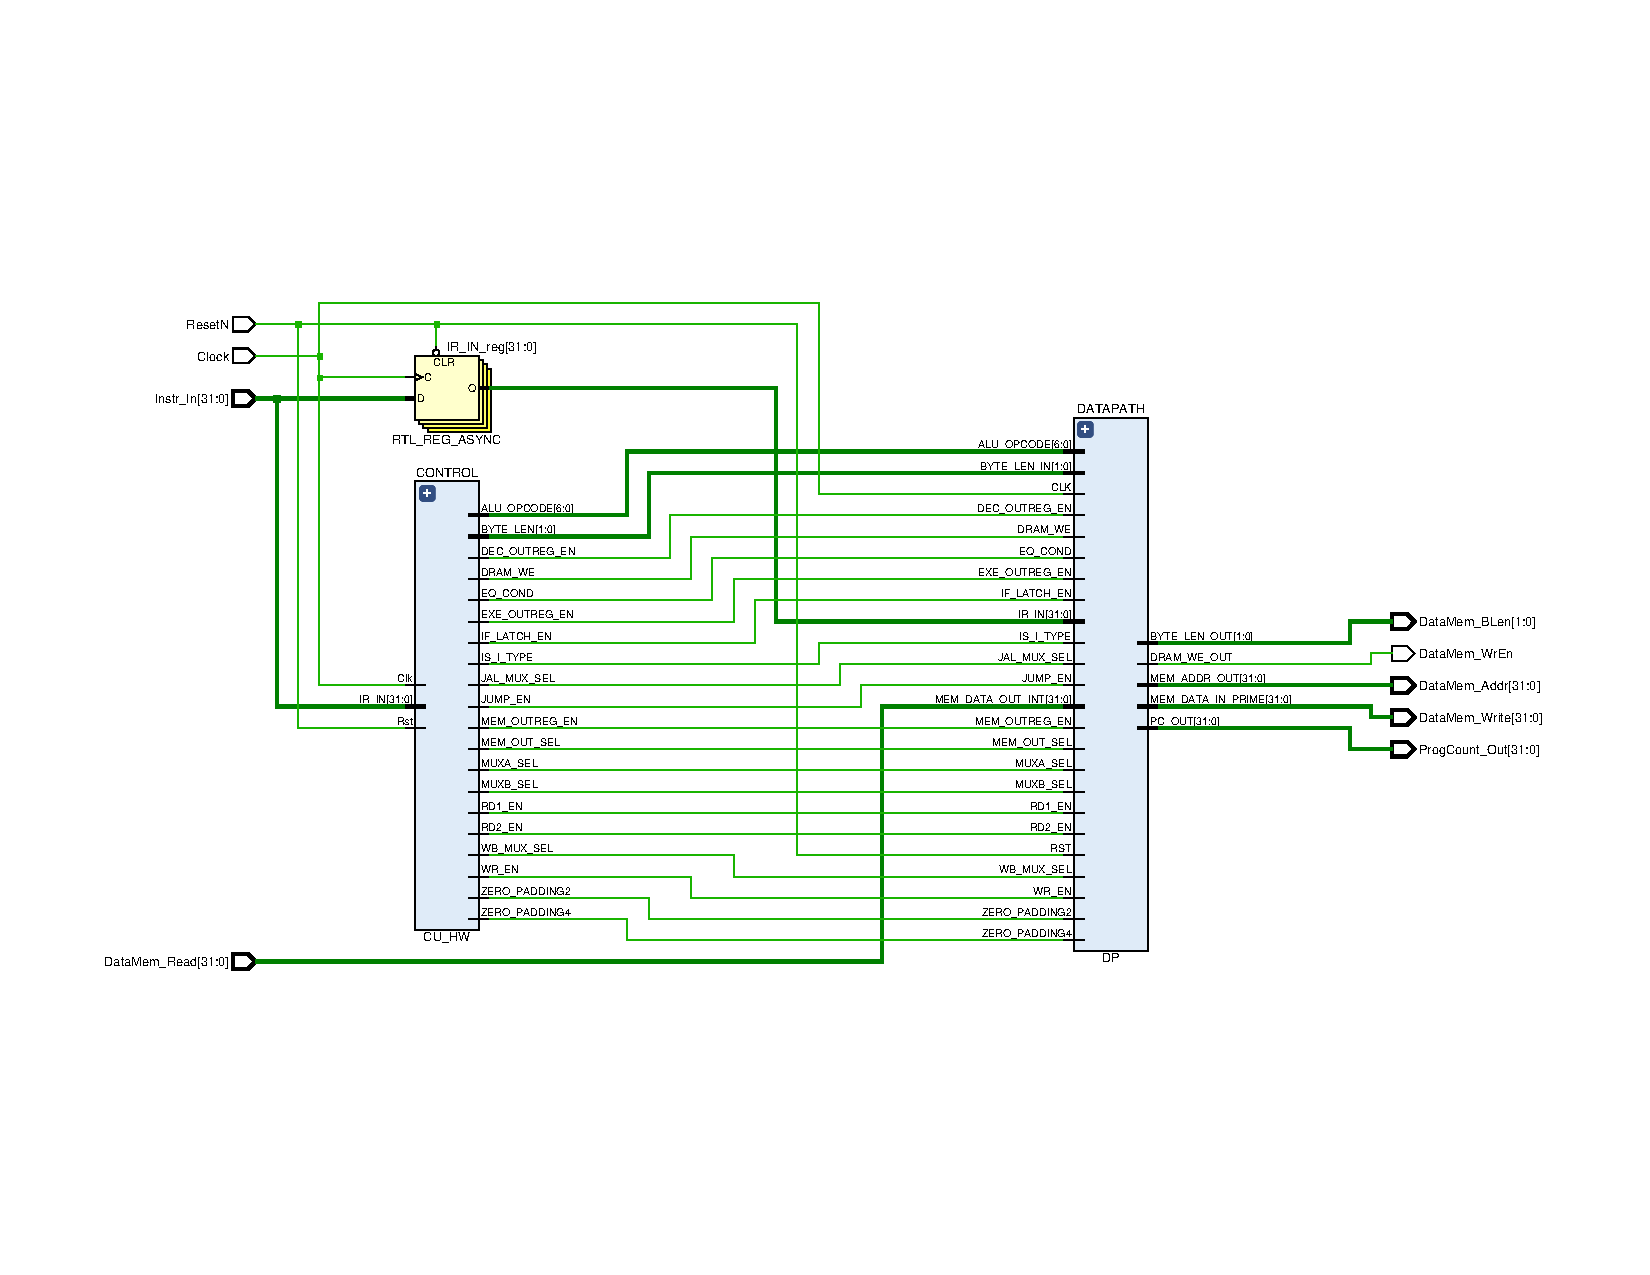
\includegraphics[width=\textwidth]{./chapters/figures/DLX.pdf} 
\caption{Top-level view of the \texttt{DLX} as a whole.}
\end{figure}

\section{Memories}
Two external Memories were used to test the design: an Instruction Memory and a Data Memory. They were implemented by strictly adhering to what's already included within the provided documentation.

\subsection{\texttt{romem}}
Used to instantiate a read-only memory that contains the set of instructions that will be fed to the microprocessor. The reset is active low and asynchronous, while reading operations are synchronous and can be delayed by any desired amount of clock cycles. The input firmware is gathered from an external text file, which must contain hexadecimals values only (once for each line).

\subsection{\texttt{rwmem}}
Instead represents a random access memory featuring the same characteristics of the previous module plus some additional capabilities. Reading is also synchronous, but now a dedicated control bus selects one format for data exchange amongst three possibilities:
\begin{table}[!ht]
\centering
\begin{tabular}{c|cc}
\toprule
\texttt{BYTE\_LEN} & Unit & Length\\
\midrule
00 & Byte & 8 bits\\
01 & Half Word & 16 bits\\
1- & Word & 32 bits\\
\bottomrule
\end{tabular}
\end{table}

An output file is finally generated with the same typesetting as the input one by means of a specialized VHDL procedure with the following prototype:
\begin{center}
\begin{BVerbatim}
rewrite_content(data, path_file)
\end{BVerbatim}
\end{center}
where \texttt{data} is the piece of information being saved, while \texttt{file\_path} is the location where those values have to be written into.

\section{Testbenches}
All the V\&V steps were handled by means of a very extensive and complete set of testbenches located inside the ``./test\_bench/'' directory. The whole assortment of components was thoroughly tested with the same bottom-up approach that was being used during the course of the implementation process.

The lower-level, more basic tests were manually compiled and carried on inside ``Mentor Graphics QuestaSim'', whereas everything starting from the ALU up was made handily available by means of a dedicated script. All these \texttt{.do} files can be found inside ``./test\_bench/scripts/'' and have to be started inside the simulator by means of the following command:
\begin{center}
\begin{BVerbatim}
do sim_MODULE.do
\end{BVerbatim}
\end{center}
where \texttt{MODULE} has to be replaced with the name of the entity in question. Additional console logs and relevant details are provided by means of assertions directly inside the GUI of the above software directly during runtime.

The only high-level block that didn't need to be tested alone was the Datapath, as its checks were directly incorporated inside \emph{TB\_DLX} after making sure that the Control Unit was 100\% functional. On that note, some relevant assembly instructions were converted into valid hexadecimal encodings by means of the provided shell script to be subsequently tested inside the aforementioned testbench.

\vspace{\baselineskip}

In order to perform a specific test suite, the user is required to copy the contents of ``./test\_bench/me\-mories/assembler/TEST\_NAME/TEST\_NAME\_dump.txt'' (where `TEST\_NAME' is a self-explanatory descriptor of the requested firmware) and paste them inside ``./memories/romem/hex.txt'' (possibly leaving \texttt{RWMEM\_DEPTH=128} lines in total), before running the usual ``sim\_DLX.do'' script. The corresponding human-readable mnemonics are located inside the \texttt{.asm} file found within the same directory as the source dump, recognized by the same test number. On the other hand, the final content of the Data Memory can be gathered from ``./test\_bench/memories/rwmem/hex.txt'' after any successful simulation.

\subsection{Known issues}
A bug inside the Memory stage was found during the final testing phase for some Load/Store instructions, and could not be fixed in time. The interface with the external Data Memory is performed in an erroneously inverse way, as the pipeline registers are located \emph{before} the combinational paths included within the same instead of synchronizing everything at the \emph{end} of it.

This causes the data to be available one clock cycle too late with respect the bits coming from the Control Unit—as such, tests \texttt{load\_store\_basic\_test} and \texttt{load\_store\_test2} cannot complete a successful run.

The best way to solve this issue would be to move the \nameref{alternate} block inside the Write Back stage, handling its control signal accordingly. This would probably even improve the regularity of the structure in question, as the subsequent \nameref{2to1} could be compacted into the final \nameref{4to1}, which in turn would actually be used to its full capacity.